\documentclass[10pt,twocolumn,letterpaper]{article}

% =========================
% Packages
% =========================
\usepackage[margin=0.75in]{geometry}
\usepackage{amsmath, amssymb, amsthm}
\usepackage{mathtools}
\usepackage{microtype}
\usepackage{graphicx}
\usepackage{subcaption}
\usepackage{booktabs}
\usepackage{multirow}
\usepackage{array}
\usepackage{tabularx}
\usepackage[hypertexnames=false]{hyperref}
\usepackage{url}
\usepackage{algpseudocode}
\usepackage{enumitem}

% =========================
% Theorem Environments
% =========================
\newtheorem{theorem}{Theorem}
\newtheorem{lemma}{Lemma}
\newtheorem{proposition}{Proposition}
\newtheorem{corollary}{Corollary}
\theoremstyle{definition}
\newtheorem{definition}{Definition}

% =========================
% Commands
% =========================
\newcommand{\R}{\mathbb{R}}
\newcommand{\Sigmahat}{\widehat{\Sigma}}
\DeclareMathOperator{\prox}{prox}
\DeclareMathOperator{\soft}{soft}
\DeclareMathOperator{\supp}{supp}
\DeclareMathOperator{\tr}{tr}
\DeclareMathOperator{\sym}{sym}
\newcolumntype{Y}{>{\raggedright\arraybackslash}X}
\setlength{\columnsep}{0.25in}
\setlength{\emergencystretch}{3em}
\hbadness=10000
\graphicspath{{figures/}}

% =========================
% Title
% =========================
\title{\texorpdfstring{Network-Constrained Sparse Principal Component Analysis: Geometric Regularization and Scalable Optimization}{Network-Constrained Sparse Principal Component Analysis: Geometric Regularization and Scalable Optimization}}
\author{Wang Zhoufu}
\date{}

\begin{document}
\sloppy
\raggedbottom
\maketitle

% =========================
% Abstract
% =========================
\begin{abstract}
Sparse principal component analysis (SPCA) improves interpretability by inducing sparse loadings, but standard formulations often treat features as exchangeable and ignore known relational structure. In many applications, including genomics, sensor networks, and finance, features are coupled by an underlying graph. We study a network-constrained SPCA formulation that combines variance maximization with an $\ell_1$ sparsity penalty and a graph Laplacian smoothness regularizer under a unit $\ell_2$ ball constraint. For this single-component problem, we identify the exact proximal map of $\lambda_1\|w\|_1 + I_{\mathbb{B}_2}(w)$ as soft-thresholding followed by radial projection, which yields a simple proximal-gradient baseline. The associated convergence statement is the standard critical-point guarantee for nonconvex composite proximal gradient under Lipschitz gradient assumptions. We also implement a multi-component block extension on the Stiefel manifold using a manifold proximal-gradient scheme with either entrywise $\ell_1$ or row-wise $\ell_{2,1}$ sparsity. The reported results remain conditional rather than uniformly dominant: in the aggregate single-component regime, $\ell_1$-SPCA attains the best mean support F1, while in a two-component synthetic study the row-sparse block method is markedly more stable than entrywise $\ell_1$ in shared-support settings and preserves orthogonality to machine precision.
\end{abstract}

% =========================
% 1. Introduction
% =========================
\section{Introduction}
Modern scientific and industrial datasets are routinely high-dimensional, with feature counts comparable to or larger than sample sizes. In this regime, dimensionality reduction is not only a computational convenience but a statistical necessity: it stabilizes estimation, reduces noise amplification, and supports interpretation. Principal component analysis (PCA) remains the canonical unsupervised approach, extracting orthogonal directions that maximize sample variance. Yet classical PCA yields dense loadings, so each component typically depends on nearly all variables, which limits interpretability and actionability in downstream tasks.

Sparse principal component analysis (SPCA) addresses this limitation by promoting sparse loadings, typically via $\ell_1$-type penalties or related sparsity-inducing regularizers. Sparsity improves interpretability by selecting a subset of variables and can reduce acquisition or monitoring costs. However, standard SPCA often treats features as exchangeable and ignores known relational structure. In many domains, this is a poor inductive bias: genes interact through pathways and regulatory networks, financial assets are coupled by sectors and supply chains, and sensors lie on physical geometries with local signal propagation. Purely sparse solutions may therefore produce fragmented supports that are statistically plausible but structurally implausible.

This paper studies \emph{network-constrained sparse PCA}, which augments SPCA with a graph Laplacian regularizer to encourage loadings that are simultaneously sparse and smooth over a feature graph. The Laplacian term penalizes local variation across graph edges and therefore favors coherent selections when the graph is informative. Our theorem-backed focus is intentionally narrow: a single-component formulation with a unit $\ell_2$ ball constraint, an exact composite proximal step, and a baseline proximal-gradient algorithm with a standard convergence guarantee. We also develop a practical multi-component extension on the Stiefel manifold and evaluate it empirically, but we do not claim a new manifold convergence theorem in this paper.

\paragraph{Contributions.}
Our main contributions are as follows:
\begin{itemize}[leftmargin=*]
  \item We formulate a graph-regularized SPCA objective that combines variance maximization, $\ell_1$ sparsity, and Laplacian smoothness under an $\ell_2$-ball constraint.
  \item We show that the update ``soft-thresholding + radial projection'' is the \emph{exact} proximal operator of $\lambda_1\|w\|_1 + I_{\mathbb{B}_2}(w)$, which yields a simple proximal-gradient baseline for the stated single-component objective.
  \item We instantiate the standard nonconvex composite proximal-gradient convergence argument for this objective and obtain convergence of the baseline method to critical points under Lipschitz gradient assumptions.
  \item We implement a multi-component block extension on the Stiefel manifold with either entrywise $\ell_1$ sparsity or row-wise $\ell_{2,1}$ sparsity, using a native manifold proximal-gradient solver with retraction-based orthogonality handling.
  \item We empirically evaluate synthetic graph families and graph-misspecification regimes, with emphasis on when graph regularization helps, when it does not, and how a practical accelerated variant changes optimization cost without changing the theorem-backed scope.
\end{itemize}
The paper does not claim a new general optimization framework, and the formal convergence theorem is restricted to the single-component baseline.

% =========================
% 2. Related Work
% =========================
\section{Related Work}
\paragraph{Sparse PCA formulations.}
A large literature studies SPCA through penalized variance maximization, regression-based formulations, matrix decomposition viewpoints, and convex relaxations; see, e.g., the original regression-based SPCA formulation in \cite{zou2006spca}, penalized matrix decomposition in \cite{witten2009pmd}, semidefinite relaxations in \cite{daspremont2007dspca}, and overview discussions in \cite{zou2018overviewSPCA}. Iterative thresholding methods such as the generalized power method provide efficient schemes for certain SPCA objectives, with strong empirical performance \cite{journee2010gpower}.

\paragraph{First-order and proximal methods.}
Motivated by scalability, recent work has emphasized first-order algorithms and proximal frameworks for structured or constrained variants of SPCA \cite{qiu2023biometrikaGradientSPCA}. Proximal gradient methods are particularly appealing for objectives comprising a smooth term plus a nonsmooth sparsity term, as the $\ell_1$ proximal operator admits a closed-form soft-thresholding map.

\paragraph{Graph-aware and network-constrained representations.}
Graph-regularized dimensionality reduction introduces Laplacian penalties to preserve geometric and relational structure. In biological and other networked settings, incorporating feature graphs has been shown to improve interpretability and scientific validity by selecting coherent modules rather than isolated variables \cite{miao2022genomeNetworkSPCA}. Our formulation is aligned with this perspective and focuses on a direct proximal-gradient treatment of a Laplacian-regularized SPCA objective under a simple norm constraint. Relative to application-specific graph PCA variants, the emphasis here is on an exact composite proximal map for the single-component objective and a careful separation between theorem-backed and practical solver variants.

\paragraph{Manifold-constrained sparse components.}
For multi-component sparse PCA, orthogonality constraints introduce Stiefel manifold geometry. In that setting, naive thresholding followed by orthogonal projection can destroy sparsity patterns, motivating manifold proximal-gradient methods that combine tangent-space proximal subproblems with retraction steps \cite{chen2020manpg,chen2020amanpg,chen2024manpgsurvey}. We use that literature to motivate a practical block manifold proximal-gradient extension with either entrywise or row-wise sparsity, while keeping our formal theorem statements restricted to the single-component Euclidean problem.

\subsection{Algorithmic Positioning and Comparison}
Table~\ref{tab:algorithm_comparison} summarizes how the proposed algorithm differs from representative SPCA solvers in objective structure, constraint geometry, and update design.

\begin{table*}[t]
\centering
\caption{Positioning of the proposed algorithm relative to representative SPCA methods.}
\label{tab:algorithm_comparison}
\small
\setlength{\tabcolsep}{4pt}
\renewcommand{\arraystretch}{1.08}
\begin{tabularx}{\textwidth}{>{\raggedright\arraybackslash}p{3.0cm}YY}
\toprule
Method family & Typical setting / update style & Key difference vs.\ this paper \\
\midrule
Generalized power / thresholding methods \cite{journee2010gpower} & Euclidean, formulation-specific power updates with truncation/thresholding & Fast and effective, but typically tied to specific SPCA objectives rather than the exact graph-composite proximal formulation analyzed here. \\
Gradient-based SPCA methods \cite{qiu2023biometrikaGradientSPCA} & Euclidean first-order methods tailored to SPCA formulations (including scalable or online settings) & Close in spirit (first-order scalability), but not the same Laplacian-regularized, unit-ball-constrained composite problem with an exact closed-form composite prox step. \\
Graph-regularized PCA/SPCA variants \cite{miao2022genomeNetworkSPCA} & Graph-aware objectives often solved by alternating or problem-specific schemes & Similar structural prior, but solver design and guarantees depend on the exact application formulation; this paper emphasizes a clean proximal-gradient derivation and theorem for the single-component case. \\
ManPG / A-ManPG \cite{chen2020manpg,chen2020amanpg} & Stiefel manifold optimization with tangent-space proximal subproblems and retractions & Natural extension for multi-component sparse orthogonal factors. More general for $V^\top V=I_k$, but more complex than the single-component Euclidean algorithm studied here. \\
\textbf{This paper (single component)} & Euclidean optimization with a unit $\ell_2$-ball constraint and graph Laplacian regularization & Exact composite proximal-gradient update (soft-thresholding + radial projection), simple implementation, and a direct convergence-to-critical-points guarantee for the stated single-component objective. \\
\bottomrule
\end{tabularx}
\end{table*}

% =========================
% 3. Problem Setup
% =========================
\section{Problem Setup}
Let $X\in\R^{n\times p}$ be centered. The sample covariance is
\begin{equation}
  \Sigmahat = \frac{1}{n}X^\top X.
\end{equation}
Let $G=(V,E)$ be a weighted undirected graph over features, with $|V|=p$, adjacency weights $\{a_{ij}\}_{(i,j)\in E}$, degree matrix $D$, and graph Laplacian $L=D-W$. Unless stated otherwise, we use this combinatorial Laplacian in both optimization and reporting. If a normalized Laplacian is used in a variant experiment, that choice should be stated explicitly because it changes both the smooth term and the reported Laplacian energy. The graph encodes prior knowledge of feature relationships.

Our goal is to learn a single sparse loading vector $w\in\R^p$ that explains variance while respecting graph structure.

\subsection{PCA and SPCA Perspective}
Classical PCA can be written either as an eigenvalue problem for $\Sigmahat$ or as a constrained matrix factorization. In high-dimensional settings, the empirical covariance is noisy and often rank-deficient, making regularization essential for stable and interpretable components. SPCA introduces sparsity to identify a parsimonious support; network-constrained SPCA further biases this support toward graph-coherent patterns.

\subsection{Graph Laplacian and Geometric Regularization}
Let $W\in\R^{p\times p}$ be a symmetric nonnegative adjacency matrix for the feature graph, and let $L=D-W$ denote the (combinatorial) Laplacian, with $D_{ii}=\sum_j W_{ij}$. The quadratic form $w^\top L w$ is the Dirichlet energy of the loading signal on the graph, and it measures local roughness. In spectral graph terms, the Laplacian eigenvectors form a graph Fourier basis: penalizing $w^\top L w$ suppresses high-frequency components of $w$ and acts as a graph low-pass regularizer. This is the geometric mechanism by which the method promotes coherent, connected supports.
This perspective is standard in spectral graph theory and graph signal processing \cite{chung1997spectral,shuman2013gsp}.

\subsection{Notation Summary}
\begin{table}[t]
\centering
\caption{Core notation used throughout the paper.}
\label{tab:notation}
\small
\begin{tabularx}{\columnwidth}{@{}lY@{}}
\toprule
Symbol & Meaning \\
\midrule
$n$ & number of samples \\
$p$ & number of features \\
$k$ & number of principal components (multi-component extension) \\
$X\in\R^{n\times p}$ & centered data matrix \\
$\Sigmahat=\frac{1}{n}X^\top X$ & sample covariance matrix \\
$G=(V,E)$ & feature graph \\
$W,D,L$ & adjacency, degree, and graph Laplacian matrices \\
$w\in\R^p$ & single-component loading vector \\
$V\in\R^{p\times k}$ & multi-component loading matrix \\
$\lambda_1,\lambda_2$ & sparsity and graph-smoothness regularization parameters \\
$\mathbb{B}_2$ & unit $\ell_2$ ball in $\R^p$ \\
\bottomrule
\end{tabularx}
\normalsize
\end{table}

% =========================
% 4. Objective
% =========================
\section{\texorpdfstring{Network-Constrained SPCA\\ Objective}{Network-Constrained SPCA Objective}}
We consider the constrained optimization problem
\begin{equation}
\label{eq:main_obj}
\max_{\|w\|_2 \le 1}\;
\underbrace{w^\top \Sigmahat w}_{\text{variance}}
\;-\;
\underbrace{\lambda_1\|w\|_1}_{\text{sparsity}}
\;-\;
\underbrace{\lambda_2 w^\top L w}_{\text{graph smoothness}},
\end{equation}
where $\lambda_1,\lambda_2\ge 0$ are tuning parameters.

\paragraph{Laplacian smoothness.}
The Laplacian quadratic form satisfies
\begin{equation}
  w^\top L w = \frac{1}{2}\sum_{(i,j)\in E} a_{ij}(w_i-w_j)^2,
\end{equation}
and thus penalizes local variation along edges. When the graph faithfully encodes relational structure, this term encourages coefficients to be similar for adjacent nodes, yielding supports that are typically more coherent and connected.

\paragraph{Composite minimization form.}
For algorithmic development, we rewrite \eqref{eq:main_obj} as minimizing
\begin{equation}
\min_{w\in\R^p} F(w)= f(w)+h(w),
\end{equation}
with
\begin{align}
  f(w) &= - w^\top \Sigmahat w + \lambda_2 w^\top L w, \\
  h(w) &= \lambda_1\|w\|_1 + I_{\mathbb{B}_2}(w),
\end{align}
where $\mathbb{B}_2=\{w:\|w\|_2\le 1\}$ and $I_{\mathbb{B}_2}$ is the indicator of the unit $\ell_2$ ball. The function $f$ is smooth (quadratic), while $h$ is proper, closed, and convex but nonsmooth.

\subsection{Multi-Component Stiefel Extension}
For $k>1$, we replace the vector loading $w$ by a loading matrix $V\in\R^{p\times k}$ and impose the orthogonality constraint
\begin{equation}
V^\top V = I_k.
\end{equation}
The corresponding block objective is
\begin{equation}
\label{eq:block_obj}
\max_{V^\top V = I_k}\;
\tr(V^\top \Sigmahat V)
\;-\;
\lambda_1 \Omega(V)
\;-\;
\lambda_2 \tr(V^\top L V),
\end{equation}
where $\Omega(V)=\|V\|_1$ gives entrywise sparsity and $\Omega(V)=\|V\|_{2,1}$ gives row sparsity shared across components.

Equivalently, we minimize
\begin{equation}
\min_{V^\top V = I_k}\; F_{\mathrm{blk}}(V)=f_{\mathrm{blk}}(V)+h_{\mathrm{blk}}(V),
\end{equation}
with
\begin{align}
f_{\mathrm{blk}}(V) &= -\tr(V^\top \Sigmahat V) + \lambda_2 \tr(V^\top L V), \\
h_{\mathrm{blk}}(V) &= \lambda_1 \Omega(V).
\end{align}
The Euclidean gradient of the smooth part is
\begin{equation}
\nabla f_{\mathrm{blk}}(V) = -2\Sigmahat V + 2\lambda_2 L V.
\end{equation}
Because the feasible set is now the Stiefel manifold, the relevant first-order direction is the Riemannian gradient
\begin{equation}
\operatorname{grad} f_{\mathrm{blk}}(V)
=
\nabla f_{\mathrm{blk}}(V) - V\,\sym\!\left(V^\top \nabla f_{\mathrm{blk}}(V)\right).
\end{equation}
This geometry prevents the single-component ``threshold then project to the ball'' update from extending directly: orthogonalization mixes coordinates and can destroy sparsity if applied naively after Euclidean thresholding.

% =========================
% 5. Optimization
% =========================
\section{Optimization Algorithm}
We apply proximal gradient to the composite objective $F=f+h$.

\subsection{Gradient of the Smooth Term}
Since $\Sigmahat$ and $L$ are symmetric,
\begin{equation}
\nabla f(w) = -2\Sigmahat w + 2\lambda_2 L w.
\end{equation}

\subsection{Composite Proximal Step}
Given step size $\eta>0$, the proximal gradient update is
\begin{equation}
  v^k = w^k - \eta \nabla f(w^k), \qquad
  w^{k+1} = \prox_{\eta h}(v^k).
\end{equation}

\paragraph{Closed-form composite proximal map.}
Although $h$ contains both the $\ell_1$ penalty and the ball indicator, the proximal map admits a simple closed form.
\begin{proposition}[Exact proximal map for $\lambda_1\|\cdot\|_1+I_{\mathbb{B}_2}$]
\label{prop:prox-composition}
Let $s=\soft(v,\eta\lambda_1)$, where $\soft$ denotes componentwise soft-thresholding. Then
\begin{equation}
\prox_{\eta h}(v)=
\begin{cases}
s, & \|s\|_2\le 1,\\
s/\|s\|_2, & \|s\|_2>1.
\end{cases}
\end{equation}
\end{proposition}

\paragraph{Derivation (sketch).}
The proximal subproblem is
\begin{equation}
\min_{\|w\|_2\le 1}\; \frac12\|w-v\|_2^2+\eta\lambda_1\|w\|_1.
\end{equation}
If the unconstrained minimizer $s=\soft(v,\eta\lambda_1)$ lies in $\mathbb{B}_2$, it is optimal. Otherwise, a KKT multiplier for the active ball constraint rescales the same soft-thresholded vector, yielding radial projection.

\paragraph{Soft-thresholding map.}
For completeness, the $\ell_1$ proximal operator is
\begin{equation}
  \soft(v^k,\eta\lambda_1)_i = \mathrm{sign}(v_i^k)\max\{|v_i^k|-\eta\lambda_1,\,0\}.
\end{equation}

\subsection{Algorithm}
\begin{figure}[t]
\centering
\caption{Proximal Gradient for Network-Constrained SPCA (Single Component)}
\label{alg:pg}
\begin{algorithmic}[1]
\Require Covariance $\Sigmahat$, Laplacian $L$, regularizers $\lambda_1,\lambda_2$, step size $\eta$, maximum iterations $K$
\State Initialize $w^0$ (e.g., leading PCA eigenvector, normalized)
\For{$k=0,1,\dots,K-1$}
  \State $g^k \gets -2\Sigmahat w^k + 2\lambda_2 L w^k$
  \State $v^k \gets w^k - \eta g^k$
  \State $s^k \gets \soft(v^k,\eta\lambda_1)$
  \If{$\|s^k\|_2>1$}
    \State $w^{k+1} \gets s^k/\|s^k\|_2$
  \Else
    \State $w^{k+1} \gets s^k$
  \EndIf
\EndFor
\State \Return $w^K$
\end{algorithmic}
\end{figure}

\paragraph{Practical step sizes.}
For quadratics, $\nabla f$ is Lipschitz with constant $L_f = 2\|-\Sigmahat + \lambda_2 L\|_2$, so $\eta\in(0,1/L_f]$ is sufficient. In practice, $\eta$ can be selected by backtracking line search to ensure monotone descent of $F$.

\subsection{Practical Solver Variant: MASPG-CAR}
Beyond Algorithm~\ref{alg:pg}, our implementation includes a practical heuristic variant, MASPG-CAR, that combines Barzilai--Borwein step initialization, monotone inertial extrapolation with restart, continuation across $(\lambda_1,\lambda_2)$, and optional active-set refinement. Its purpose is to reduce repeated-solve cost over hyperparameter paths while preserving the same exact composite proximal map.

\paragraph{Scope of guarantees.}
MASPG-CAR is not covered by the theorem below. In this paper it is treated strictly as an engineering comparison against the baseline proximal-gradient solver. The experimental section therefore reports it only through empirical iteration and runtime differences, together with any change in solution quality.

\subsection{Block Manifold Proximal Gradient}
For the multi-component objective \eqref{eq:block_obj}, we use a practical block manifold proximal-gradient method. Starting from an orthonormal loading matrix $V^t$, the algorithm:
\begin{enumerate}[leftmargin=*]
\item computes the Riemannian gradient of the smooth block objective;
\item takes a gradient step in the ambient space;
\item applies either entrywise soft-thresholding ($\ell_1$ mode) or row-group shrinkage ($\ell_{2,1}$ mode);
\item retracts the result back to the Stiefel manifold using a polar retraction, with QR as fallback.
\end{enumerate}

The resulting update can be written schematically as
\begin{align}
G^t_{\mathrm{R}} &= \operatorname{grad} f_{\mathrm{blk}}(V^t), \\
Y^t &= V^t - \eta_t G^t_{\mathrm{R}}, \\
Z^t &= \prox_{\eta_t \lambda_1 \Omega}(Y^t), \\
V^{t+1} &= \operatorname{Retr}(Z^t),
\end{align}
with monotone backtracking on the full block objective. In $\ell_1$ mode, $\prox_{\eta_t \lambda_1 \Omega}$ is entrywise soft-thresholding. In $\ell_{2,1}$ mode, each row is shrunk by the usual group soft-thresholding rule. The implementation logs objective decrease, step size, relative iterate change, Riemannian gradient norm, support size, and orthogonality error.

\begin{figure}[t]
\centering
\caption{Block Manifold Proximal Gradient for Multi-Component NC-SPCA}
\label{alg:block_manpg}
\begin{algorithmic}[1]
\Require Data matrix $X$, Laplacian $L$, regularizers $\lambda_1,\lambda_2$, component count $k$, initial orthonormal $V^0$
\For{$t=0,1,\dots,K-1$}
  \State $G^t \gets -2\Sigmahat V^t + 2\lambda_2 L V^t$
  \State $G^t_{\mathrm{R}} \gets G^t - V^t \frac{(V^t)^\top G^t + (G^t)^\top V^t}{2}$
  \State $Y^t \gets V^t - \eta_t G^t_{\mathrm{R}}$
  \State $Z^t \gets \prox_{\eta_t \lambda_1 \Omega}(Y^t)$
  \State $V^{t+1} \gets \operatorname{Retr}(Z^t)$
  \State update $\eta_t$ by monotone backtracking if needed
\EndFor
\State \Return $V^K$
\end{algorithmic}
\end{figure}

\paragraph{Scope of guarantees.}
Algorithm~\ref{alg:block_manpg} is a practical manifold extension motivated by ManPG-type methods, but this paper does not claim a new convergence theorem for it. Our claims for the block method are therefore empirical: orthogonality preservation, recovery behavior under different sparsity structures, and runtime characteristics in controlled synthetic settings.

% =========================
% 6. Convergence
% =========================
\section{Convergence Analysis}
Because Proposition~\ref{prop:prox-composition} identifies the exact proximal map of $h$, Algorithm~\ref{alg:pg} is a standard proximal-gradient method for a nonconvex composite objective with smooth part $f$ and convex nonsmooth part $h$.

\subsection{Assumptions}
\begin{definition}[Lipschitz gradient]
A differentiable function $f$ has $L_f$-Lipschitz continuous gradient if
\begin{equation}
\|\nabla f(u)-\nabla f(v)\|_2 \le L_f\|u-v\|_2,\qquad \forall u,v\in\R^p.
\end{equation}
\end{definition}

\paragraph{Assumption 1.}
The function $f(w)=-w^\top \Sigmahat w + \lambda_2 w^\top L w$ has Lipschitz continuous gradient with constant $L_f$.

\paragraph{Assumption 2.}
The step size satisfies $0<\eta<1/L_f$ (or is selected by a descent-preserving line search).

\subsection{Stationarity}
\begin{definition}[Critical point]
A point $w^\star$ is a critical point of $F(w)=f(w)+h(w)$ if it satisfies the first-order optimality condition
\begin{equation}
0 \in \nabla f(w^\star) + \partial h(w^\star),
\end{equation}
equivalently,
\begin{equation}
0 \in \nabla f(w^\star) + \lambda_1\partial\|w^\star\|_1 + N_{\mathbb{B}_2}(w^\star),
\end{equation}
where $N_{\mathbb{B}_2}(w^\star)$ denotes the normal cone of the unit $\ell_2$ ball at $w^\star$.
\end{definition}

\subsection{Baseline PG Guarantee}
\begin{theorem}[Convergence to critical points]
\label{thm:conv}
Suppose Assumptions 1--2 hold. Then the sequence $\{w^k\}$ generated by Algorithm~\ref{alg:pg} satisfies:
\begin{enumerate}[leftmargin=*]
\item The objective values $\{F(w^k)\}$ are non-increasing.
\item $\|w^{k+1}-w^k\|_2 \to 0$ as $k\to\infty$.
\item Every accumulation point (cluster point) of $\{w^k\}$ is a critical point of $F$.
\end{enumerate}
\end{theorem}

\paragraph{Proof sketch.}
The proof uses the standard descent lemma for smooth functions and the characterization of the proximal-gradient step as minimizing a local quadratic upper bound of $f$ plus $h$. By Proposition~\ref{prop:prox-composition}, the implemented update is exactly this proximal-gradient step. Under Lipschitz continuity of $\nabla f$ and a sufficiently small step size, one obtains a sufficient-decrease inequality and summability of $\|w^{k+1}-w^k\|_2^2$, which implies asymptotic regularity. Criticality of accumulation points follows from standard limiting-subdifferential arguments for nonconvex composite minimization.

\paragraph{Interpretation.}
Theorem~\ref{thm:conv} is a standard proximal-gradient result instantiated for the specific objective in this paper. The technical interest here is not a new convergence paradigm, but the fact that the exact composite proximal step makes the baseline method particularly simple to implement for the graph-regularized ball-constrained objective.

\paragraph{Stability note (multi-component extensions).}
For multiple components with an orthogonality constraint $V^\top V=I_k$, naive thresholding followed by orthogonal projection generally destroys sparsity. The empirical block method used in this paper controls that issue through retraction-based manifold updates and maintains numerical orthogonality at machine precision in the reported synthetic runs, but its convergence is not covered by Theorem~\ref{thm:conv}.

\paragraph{Remark on global convergence statements.}
For manifold variants and alternating schemes, convergence claims typically require assumptions beyond Lipschitz smoothness (e.g., sufficient decrease and a suitable regularity/KL-type property). Accordingly, this paper restricts formal theorem statements to the single-component composite proximal-gradient algorithm above and treats manifold methods as principled extensions rather than proved results in this document.

% =========================
% 7. Experiments
% =========================
\section{Experimental Study}
We evaluate whether incorporating network structure improves \emph{structured feature selection} and \emph{support recovery} relative to unstructured alternatives while preserving explained variance. The working hypothesis is conditional: graph regularization should help when the graph is informative and can fail when the graph is misspecified.

\subsection{Synthetic Data and Graph Families}
We generate feature graphs $G$ from several families:
(i) chains (contiguous supports),
(ii) grids (spatial structure),
(iii) random geometric graphs (local neighborhoods),
(iv) stochastic block models (community structure).
We construct ground-truth sparse loadings with connected support sets (when appropriate) and sample data from a spiked covariance model whose leading component aligns with the ground truth. This design isolates the effect of graph regularization on recovery while keeping the data-generating process controlled. It also makes failure modes easier to interpret because both the true support and the estimator graph are known.

\subsection{Data-Generating Process}
For a graph $G$ on $p$ nodes, let $S^\star\subseteq\{1,\dots,p\}$ denote a connected support set of size $s$. We define a ground-truth loading $w^\star\in\R^p$ with $\supp(w^\star)=S^\star$ and $\|w^\star\|_2=1$ (e.g., piecewise-smooth values over $S^\star$). A simple spiked covariance model is
\begin{equation}
\Sigma^\star = \sigma^2 I_p + \beta\, w^\star (w^\star)^\top,
\end{equation}
with signal strength $\beta>0$ and noise level $\sigma^2>0$. Data are generated as $x_i\sim \mathcal{N}(0,\Sigma^\star)$ for $i=1,\dots,n$, and the centered design matrix $X$ is formed from the samples.

\paragraph{Graph-quality stress tests.}
To study robustness, we also perturb the feature graph used by the estimator while keeping $\Sigma^\star$ fixed. The misspecification table below corresponds to edge perturbation at rate $0.1$, which directly probes sensitivity to graph mismatch.

\subsection{Reported Protocol}
The aggregate benchmark tables are taken from the tracked paper-audit run over the four graph families above with three repeats per family and fixed regularization parameters $\lambda_1=0.15$ and $\lambda_2=0.25$. The optimization ablation compares baseline PG and MASPG-CAR over ten repeated synthetic runs under shared initialization and stopping rules. Separate chain-graph sweeps are used only for tradeoff visualization.

\paragraph{Block-study protocol.}
The multi-component results reported below use the native block manifold proximal-gradient implementation with $k=2$ components and five repeats per regime. We report four block regimes that are directly supported by the current code path: `grid/disjoint', `chain/shared', `rgg/disjoint', and `sbm/disjoint'. Unless stated otherwise, these runs use $n=60$, signal strength $\beta=8$, noise standard deviation $1$, $\lambda_1=0.15$, $\lambda_2=0.25$, and polar retraction.

\paragraph{Reproducible protocol details.}
The reported runs fix the following:
\begin{itemize}[leftmargin=*]
\item graph families $\{$chain, grid, random geometric graph, SBM$\}$;
\item three repeats per family for the aggregate audit tables;
\item ten repeats for the PG vs.\ MASPG-CAR optimizer ablation;
\item support extraction threshold $10^{-6}$;
\item the combinatorial Laplacian in both optimization and reported Laplacian energy.
\end{itemize}

\paragraph{Tradeoff sweep used for figures.}
The two sweep figures in this section come from a chain-graph run with $n=200$, $p=100$, support size $20$, signal strength $\beta=8$, noise standard deviation $1$, and a small grid over $\lambda_1\in\{0.1,0.2\}$ and $\lambda_2\in\{0,0.1\}$.

\subsection{Baselines}
We compare:
\begin{itemize}[leftmargin=*]
\item PCA,
\item $\ell_1$-SPCA (no graph regularization; $\lambda_2=0$),
\item graph-regularized PCA (no sparsity; $\lambda_1=0$),
\item the proposed method (graph regularization and sparsity).
\end{itemize}
For the multi-component study, the comparison is internal to the native block solver: entrywise $\ell_1$ sparsity versus row-wise $\ell_{2,1}$ sparsity under the same graph, initialization, and stopping rules.

\subsection{Implementation and Scalability Considerations}
For large $p$, each iteration is dominated by matrix-vector products with $\Sigmahat$ and $L$, plus the $O(p)$ soft-thresholding operation. When $L$ is sparse and $\Sigmahat w$ is computed implicitly via $X^\top(Xw)/n$, the method scales well to high-dimensional regimes. This structure also supports warm starts across a regularization path and straightforward parallelization across simulation replicates.

\paragraph{Per-iteration complexity (implicit covariance implementation).}
If $X$ is stored explicitly, computing $\Sigmahat w = X^\top(Xw)/n$ costs $O(np)$, and multiplying by a sparse Laplacian costs $O(|E|)$. Thus each iteration is approximately $O(np + |E|)$ plus lower-order vector operations. This makes the method practical when $k=1$ and the graph is sparse, even for large $p$.

\subsection{Optimizer Ablation}
The practical-variant comparison is restricted to baseline PG versus MASPG-CAR. Both solvers use the same objective, initialization policy, support-thresholding rule, and stopping tolerance, so any difference is attributable to the acceleration heuristics rather than to a changed objective or post-processing pipeline.

\subsection{Evaluation Metrics}
We report:
\begin{itemize}[leftmargin=*]
\item explained variance $w^\top \Sigmahat w$,
\item support recovery (precision/recall/F1 against the true support),
\item structural coherence (largest connected-component ratio and Laplacian energy $w^\top L w$ within the selected support),
\item runtime and iteration counts.
\end{itemize}
For the multi-component study, we additionally report permutation-invariant matched-support F1 across components, shared-support F1, and orthogonality error $\|V^\top V-I\|_F$.

\subsection{Results}
\begin{table}[t]
\centering
\caption{Aggregate synthetic benchmark results for the tracked synthetic study. Values are means across chain, grid, random geometric graph, and SBM families.}
\label{tab:main_performance}
\scriptsize
\setlength{\tabcolsep}{3pt}
\begin{tabularx}{\columnwidth}{@{}l>{\centering\arraybackslash}X>{\centering\arraybackslash}X>{\centering\arraybackslash}X>{\centering\arraybackslash}X@{}}
\toprule
Method & Var.\ Explained $\uparrow$ & F1 $\uparrow$ & LCC Ratio $\uparrow$ & Time (s) $\downarrow$ \\
\midrule
PCA & 9.899 & 0.337 & 1.000 & 0.0027 \\
$\ell_1$-SPCA & 9.857 & 0.403 & 0.998 & 0.0074 \\
Graph-PCA & 9.830 & 0.336 & 1.000 & 0.0092 \\
NetSPCA-PG & 9.799 & 0.397 & 0.995 & 0.0094 \\
NetSPCA-MASPG-CAR & 9.797 & 0.397 & 0.995 & 0.0090 \\
\bottomrule
\end{tabularx}
\normalsize
\end{table}

\begin{table}[t]
\centering
\caption{Aggregate synthetic benchmark results under graph misspecification (edge perturbation rate $0.1$).}
\label{tab:misspec_performance}
\scriptsize
\setlength{\tabcolsep}{3pt}
\begin{tabularx}{\columnwidth}{@{}l>{\centering\arraybackslash}X>{\centering\arraybackslash}X>{\centering\arraybackslash}X>{\centering\arraybackslash}X@{}}
\toprule
Method & Var.\ Explained $\uparrow$ & F1 $\uparrow$ & LCC Ratio $\uparrow$ & Time (s) $\downarrow$ \\
\midrule
PCA & 9.410 & 0.338 & 1.000 & 0.0028 \\
$\ell_1$-SPCA & 9.367 & 0.419 & 1.000 & 0.0076 \\
Graph-PCA & 9.234 & 0.335 & 1.000 & 0.0096 \\
NetSPCA-PG & 9.222 & 0.403 & 1.000 & 0.0094 \\
NetSPCA-MASPG-CAR & 9.221 & 0.403 & 1.000 & 0.0087 \\
\bottomrule
\end{tabularx}
\normalsize
\end{table}

\paragraph{Primary empirical finding.}
In the reported aggregate regime, $\ell_1$-SPCA achieves the highest mean support F1 among the core methods in both the base benchmark ($0.403$) and the misspecified-graph benchmark ($0.419$). The network-constrained variants remain close in F1 in the base setting ($0.397$) but do not exceed the unstructured sparse baseline, and the gap widens under graph misspecification ($0.403$ versus $0.419$). The aggregate LCC ratios are already near one for all sparse methods, so these tables do not support a strong claim of coherence gains in this regime.

\begin{figure*}[t]
\centering
\begin{subfigure}[t]{0.48\textwidth}
  \centering
  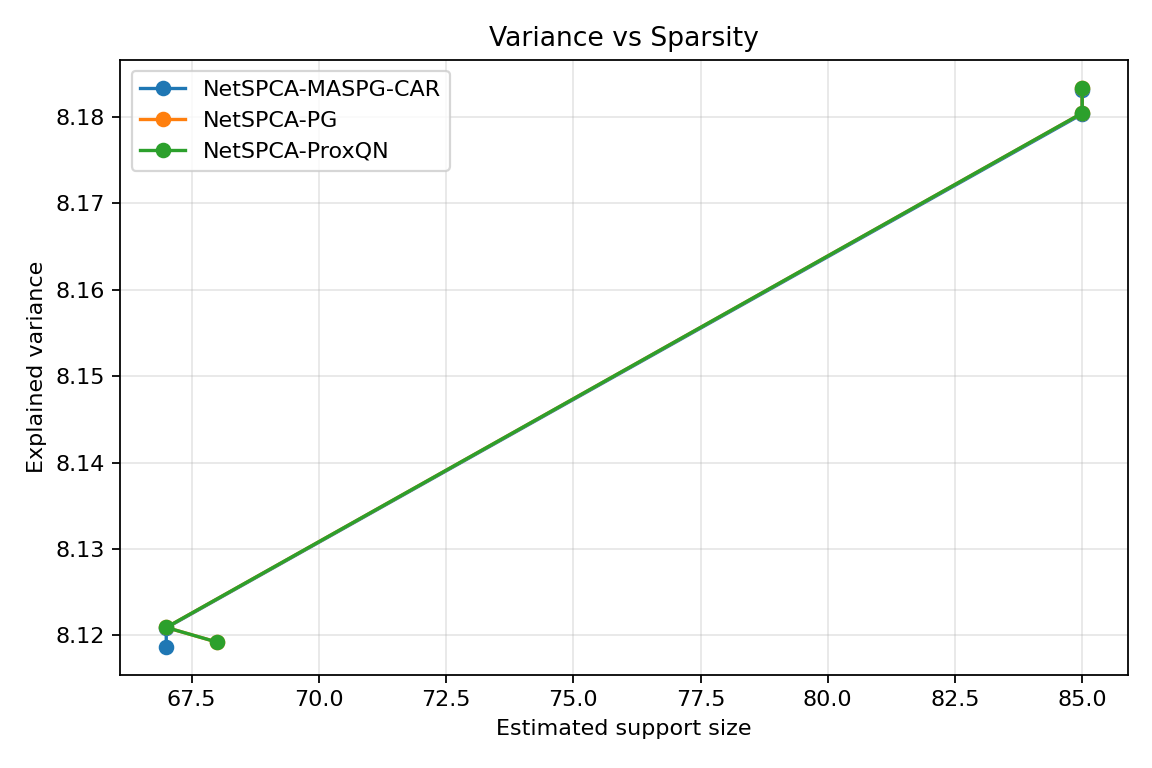
\includegraphics[width=\textwidth]{variance_vs_sparsity.png}
  \caption{Explained variance versus estimated support size in the chain-graph sweep.}
\end{subfigure}
\hfill
\begin{subfigure}[t]{0.48\textwidth}
  \centering
  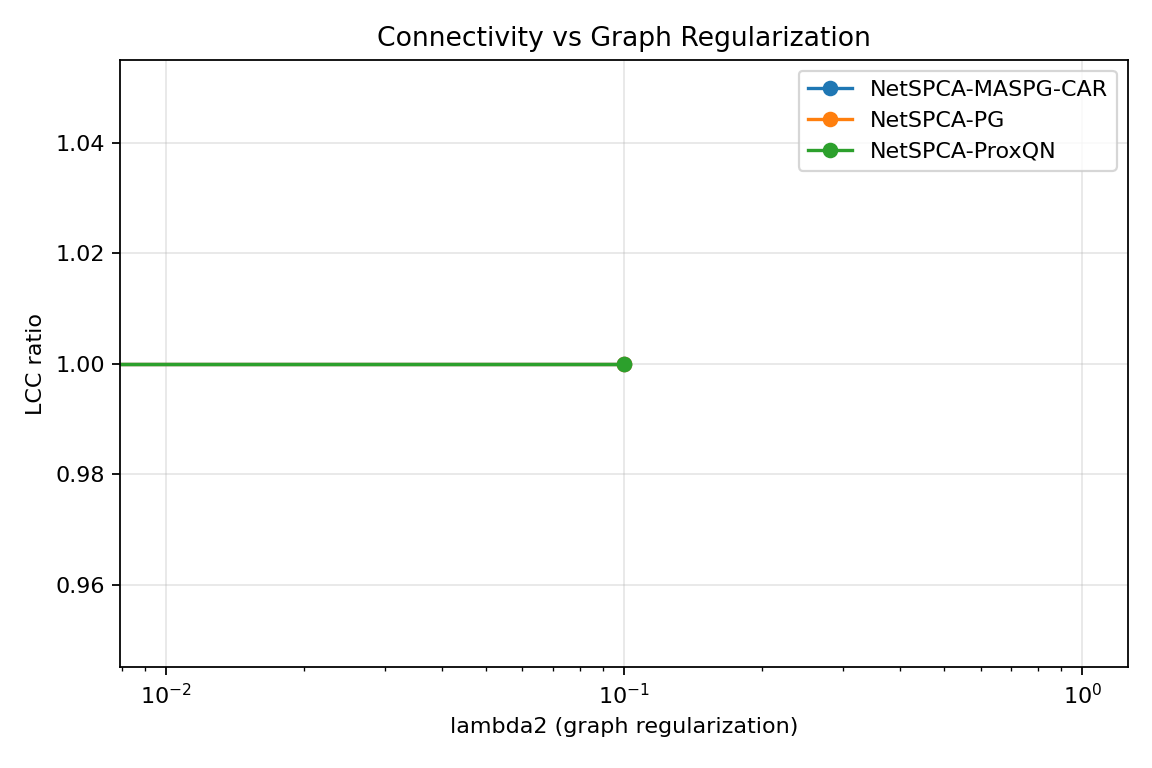
\includegraphics[width=\textwidth]{connectivity_vs_lambda2.png}
  \caption{LCC ratio versus $\lambda_2$ in the same sweep.}
\end{subfigure}
\caption{Measured tradeoff sweep for the chain-graph setting with $n=200$, $p=100$, support size $20$, signal strength $\beta=8$, and $\lambda_1\in\{0.1,0.2\}$, $\lambda_2\in\{0,0.1\}$. The sweep exposes the intended sparsity--variance tradeoff, but the connectivity metric remains saturated at one in this regime, so it does not provide evidence of a substantial aggregate coherence gain.}
\label{fig:tradeoff_sweeps}
\end{figure*}

\paragraph{Tradeoff interpretation.}
Figure~\ref{fig:tradeoff_sweeps} makes the same point from a parameter-sweep perspective. In the present chain-graph sweep, increasing sparsity changes support size and explained variance in the expected direction, but increasing $\lambda_2$ does not yield a visible connectivity gain because the selected supports are already connected across the tested settings. The useful operating regime is therefore a Pareto region rather than a single universally superior parameter pair, and its location depends on graph quality.

\begin{figure}[t]
\centering
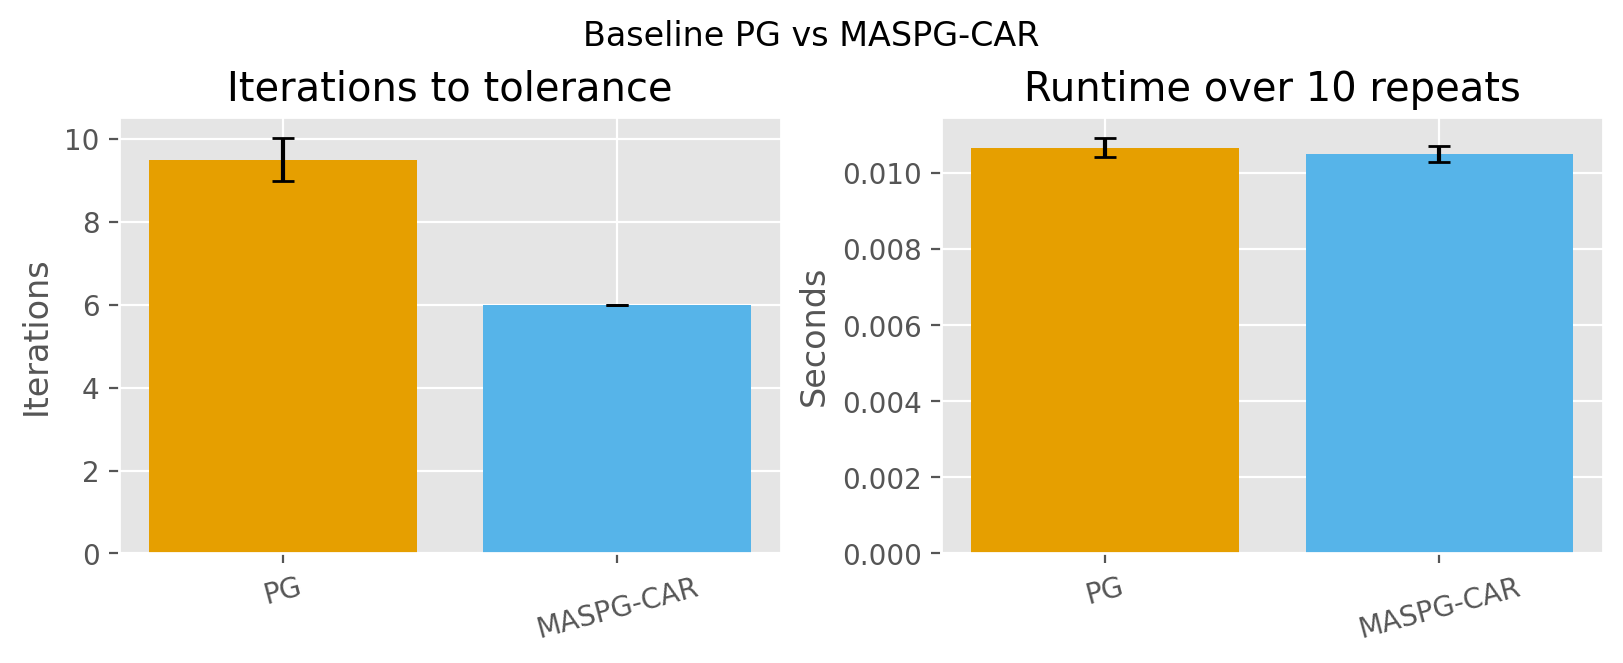
\includegraphics[width=\columnwidth]{optimizer_ablation.png}
\caption{Baseline PG versus MASPG-CAR over ten repeated synthetic runs. Error bars show sample standard deviations. MASPG-CAR reduces the iteration count from $9.5\pm0.53$ to $6.0\pm0.0$, while mean runtime changes only slightly from $0.01067\pm0.00026$ s to $0.01050\pm0.00022$ s.}
\label{fig:optimizer_ablation}
\end{figure}

\paragraph{Practical optimization finding.}
Figure~\ref{fig:optimizer_ablation} shows that MASPG-CAR is best understood as an engineering heuristic. In the audited ten-repeat comparison, it reduces iterations substantially, but the wall-clock effect is modest and support F1 is statistically indistinguishable from baseline PG. The continuation path experiment remains the clearest measured runtime gain, reducing total path iterations from $136$ to $91$ in the tracked sweep.

\subsection{Multi-Component Block Results}
\begin{table*}[t]
\centering
\caption{Two-component block NC-SPCA results for the native manifold proximal-gradient implementation. Means are over five repeats. The `grid/disjoint' regime uses a $4\times4$ grid with two disjoint supports of size four. The `chain/shared' regime uses a length-20 chain with two components sharing the same support. The `rgg/disjoint' and `sbm/disjoint' regimes use random geometric and stochastic block-model graphs with disjoint supports of size four.}
\label{tab:block_results}
\small
\setlength{\tabcolsep}{4pt}
\renewcommand{\arraystretch}{1.08}
\begin{tabularx}{\textwidth}{@{}l l >{\centering\arraybackslash}p{1.5cm} >{\centering\arraybackslash}p{1.5cm} >{\centering\arraybackslash}p{1.5cm} >{\centering\arraybackslash}p{1.4cm} >{\centering\arraybackslash}p{1.6cm} >{\centering\arraybackslash}p{1.5cm}@{}}
\toprule
Regime & Sparsity & Matched F1 $\uparrow$ & Shared F1 $\uparrow$ & Mean LCC $\uparrow$ & Conv.\ Rate $\uparrow$ & Iterations $\downarrow$ & Time (s) $\downarrow$ \\
\midrule
grid/disjoint & $\ell_1$ & 0.400 & 0.667 & 1.000 & 1.00 & 130.4 & 0.0289 \\
grid/disjoint & $\ell_{2,1}$ & 0.400 & 0.667 & 1.000 & 1.00 & 28.0 & 0.0066 \\
chain/shared & $\ell_1$ & 0.344 & 0.342 & 0.768 & 0.40 & 346.6 & 0.0697 \\
chain/shared & $\ell_{2,1}$ & 0.339 & 0.339 & 0.821 & 1.00 & 168.6 & 0.0407 \\
rgg/disjoint & $\ell_1$ & 0.289 & 0.494 & 0.398 & 0.80 & 243.4 & 0.0572 \\
rgg/disjoint & $\ell_{2,1}$ & 0.278 & 0.488 & 0.395 & 1.00 & 46.6 & 0.0113 \\
sbm/disjoint & $\ell_1$ & 0.293 & 0.510 & 0.789 & 1.00 & 200.0 & 0.0513 \\
sbm/disjoint & $\ell_{2,1}$ & 0.288 & 0.503 & 0.798 & 1.00 & 46.6 & 0.0178 \\
\bottomrule
\end{tabularx}
\normalsize
\end{table*}

\paragraph{Block-method interpretation.}
Table~\ref{tab:block_results} shows a clear regime dependence, but also a consistent optimization pattern. In the disjoint-support grid setting, entrywise $\ell_1$ and row-wise $\ell_{2,1}$ give the same matched-support and shared-support scores, but $\ell_{2,1}$ reaches that solution much faster, reducing mean iterations from $130.4$ to $28.0$. In the shared-support chain setting, the tradeoff changes: entrywise $\ell_1$ attains a slightly larger matched-support F1, but it converges in only $40\%$ of runs and has lower structural coherence. The row-sparse $\ell_{2,1}$ model converges in all runs, improves mean component connectivity from $0.768$ to $0.821$, and roughly halves both iteration count and runtime. The broader disjoint-support runs on random geometric and stochastic block-model graphs follow the same pattern: $\ell_{2,1}$ trades a small amount of matched-support F1 for materially better convergence behavior and substantially lower runtime. Across all eight settings, the orthogonality error remained at machine precision, with mean $\|V^\top V-I\|_F$ between $4.5\times 10^{-16}$ and $9.1\times 10^{-16}$.

\begin{figure*}[t]
\centering
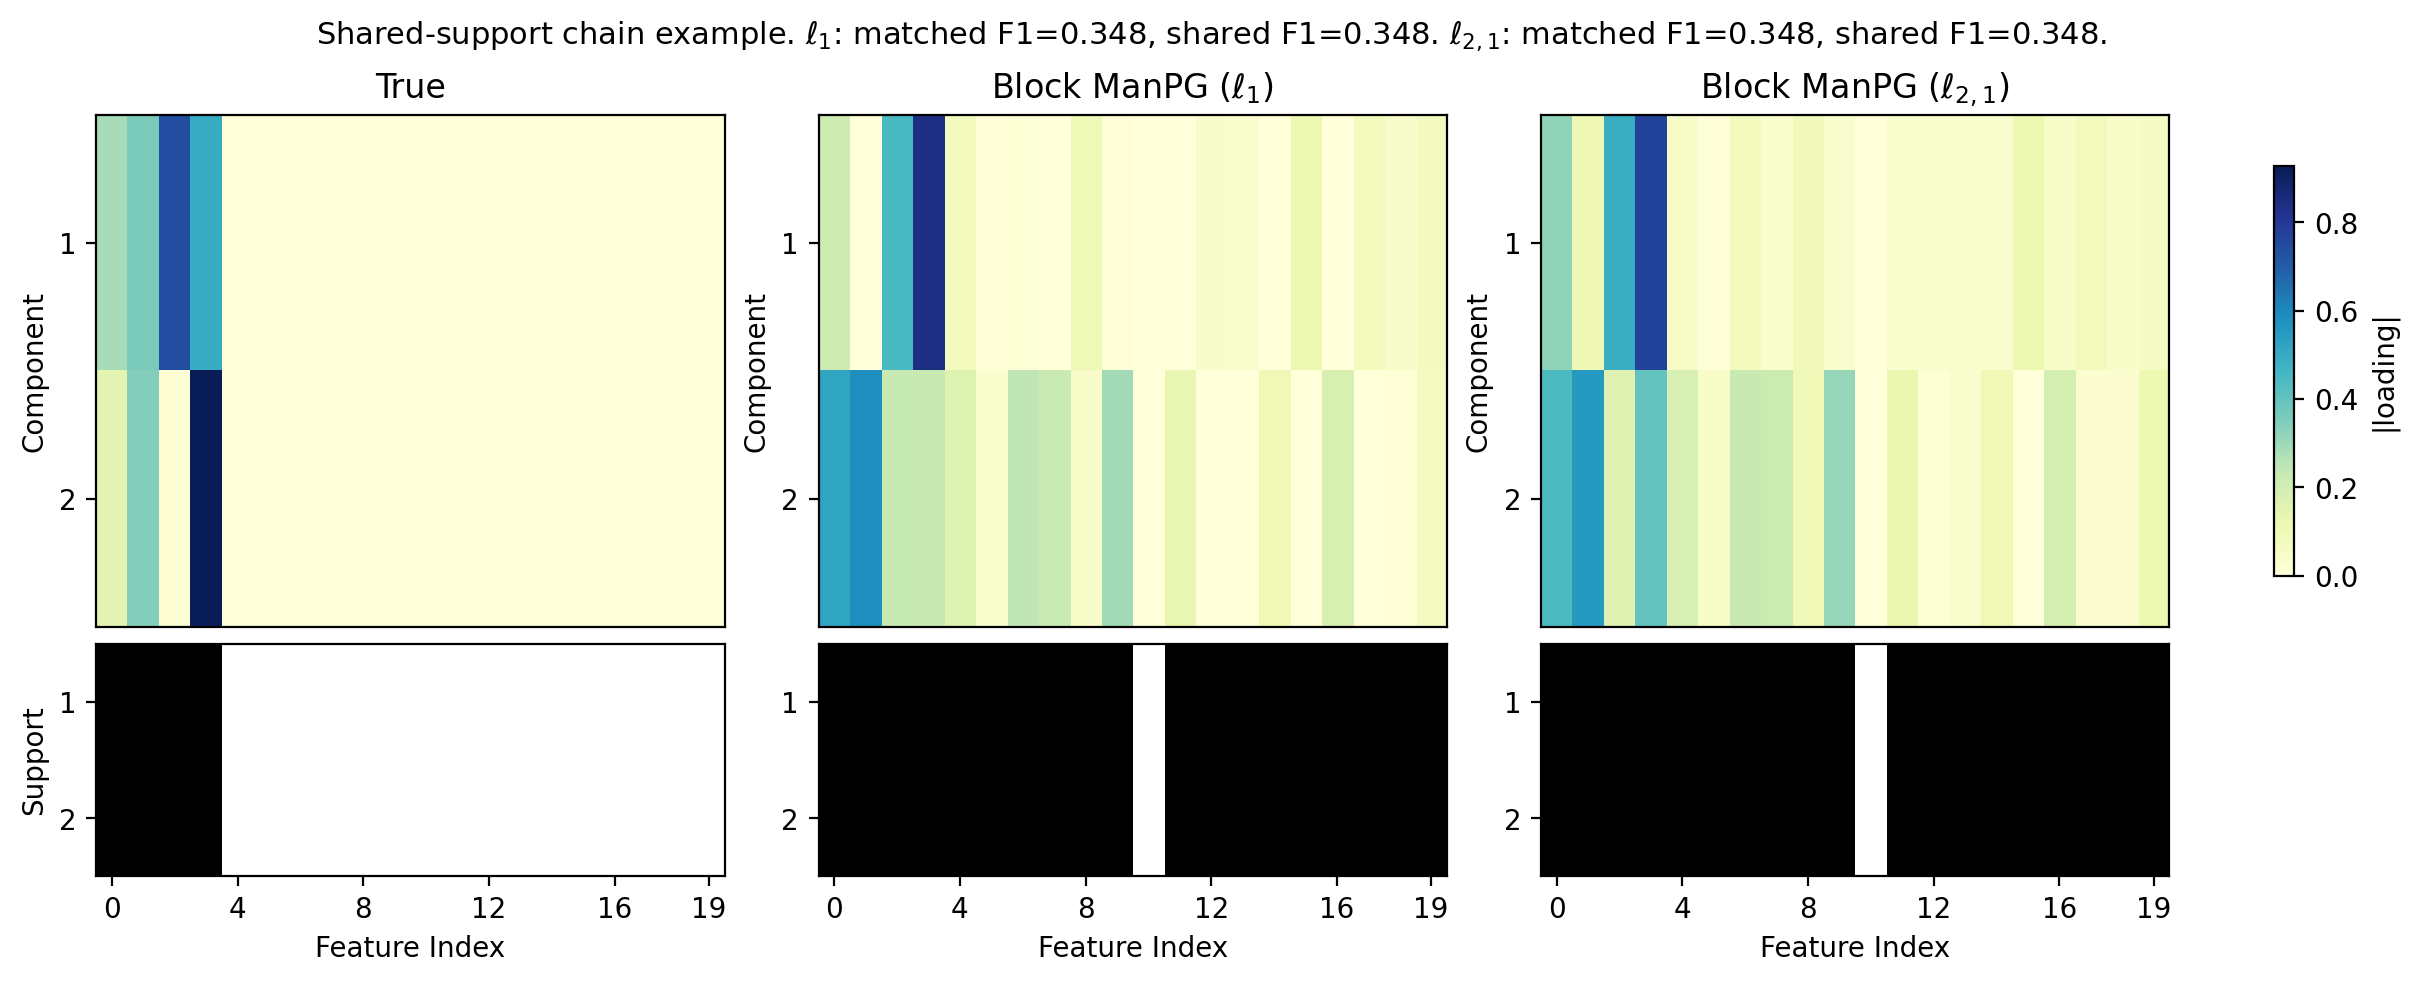
\includegraphics[width=0.92\textwidth]{block_support_patterns.png}
\caption{Fixed-seed shared-support chain example for the block method. The top row shows absolute loadings for the true loading matrix, the entrywise $\ell_1$ fit, and the row-sparse $\ell_{2,1}$ fit. The bottom row shows the corresponding thresholded supports. In this regime, the two components share the same true support. The row-sparse model preserves that structural bias more directly, whereas the entrywise model yields a more fragmented support pattern even when matched-support F1 remains similar.}
\label{fig:block_support_patterns}
\end{figure*}

\paragraph{Qualitative support pattern.}
Figure~\ref{fig:block_support_patterns} shows the regime in which the choice of sparsity model matters most. When the latent components truly share variables, the row-sparse formulation better reflects that inductive bias by suppressing isolated row activations. This is the main interpretive benefit of the block extension: not a universal F1 improvement, but a better alignment between the estimated support pattern and the structural prior encoded by the model class.

% =========================
% 8. Discussion
% =========================
\section{Discussion and Limitations}
\paragraph{Graph quality and misspecification.}
The Laplacian regularizer improves structural coherence only when the feature graph is informative. Misspecified, noisy, or overly dense graphs can induce over-smoothing, blur support boundaries, and degrade recovery. In practice, graph preprocessing (thresholding, normalization, confidence weighting) can materially affect results and should be documented.

\paragraph{Single-component vs.\ multi-component formulations.}
Our formal algorithmic and convergence results target a single component under an $\ell_2$-ball constraint. The multi-component extension introduces orthogonality constraints and a different geometry, so its method class is necessarily different. The present block experiments show that a native manifold proximal-gradient implementation is workable and numerically stable, but they also show that the preferred sparsity pattern depends on the scientific question: entrywise $\ell_1$ is competitive for disjoint supports, whereas row-wise $\ell_{2,1}$ is materially more stable when components are expected to share variables.

\paragraph{High-dimensional inference and uncertainty quantification.}
Optimization convergence alone does not imply statistical consistency or valid uncertainty quantification. In high-dimensional settings, inferential guarantees depend on signal strength, graph quality, regularization scaling, and model mismatch. A complete inference theory for graph-regularized SPCA (e.g., support recovery guarantees and perturbation bounds under graph misspecification) remains an important research direction.

\paragraph{Applications and implications.}
The framework is well motivated in genomics, finance, and sensor networks, where domain knowledge naturally induces feature graphs. In such settings, network-constrained SPCA can be viewed as a structured feature selection mechanism that trades off variance explanation against geometric coherence. Its practical value depends on whether the graph captures stable domain structure rather than transient correlations. The reported synthetic study supports the caution that graph-based methods are not uniformly dominant under misspecification.

% =========================
% 9. Conclusion
% =========================
\section{Conclusion}
We studied a network-constrained SPCA objective that jointly promotes variance explanation, sparsity, and graph smoothness through a graph Laplacian regularizer. For the single-component, $\ell_2$ ball constrained formulation, the resulting method is a simple proximal-gradient algorithm with a closed-form composite proximal map and a standard convergence guarantee to critical points. We also implemented a multi-component Stiefel-manifold extension and reported its empirical behavior under entrywise and row-structured sparsity.

The main practical implication is that structural priors can be integrated into sparse dimensionality reduction without sacrificing first-order scalability. The main empirical caveat is that this structural bias is conditionally useful rather than uniformly superior: in the present aggregate single-component regime, $\ell_1$-SPCA remains the strongest support-recovery baseline, and in the block regime the best sparsity model depends on whether supports are shared across components. Future work should develop statistical recovery guarantees under graph misspecification, robust graph learning variants, and a full convergence analysis for the block manifold proximal-gradient method used here.

% =========================
% Appendix
% =========================
\appendix

\section{Appendix: Proof and Derivation Details}
\subsection{Proof of Proposition~\ref{prop:prox-composition} (Expanded)}
Let $\tau=\eta\lambda_1$ and consider
\begin{equation}
\label{eq:appendix_prox_problem}
\min_{\|w\|_2\le 1}\; \phi(w):=\frac12\|w-v\|_2^2+\tau\|w\|_1.
\end{equation}
Because $\phi$ is convex and the constraint set $\mathbb{B}_2$ is closed and convex, a minimizer exists and KKT conditions are necessary and sufficient. Thus $w^\star$ solves \eqref{eq:appendix_prox_problem} iff there exists $\mu^\star\ge 0$ such that
\begin{align}
0 &\in w^\star - v + \tau \partial\|w^\star\|_1 + \mu^\star w^\star, \label{eq:kkt_stationarity}\\
\mu^\star(\|w^\star\|_2-1)&=0, \qquad \|w^\star\|_2\le 1. \label{eq:kkt_complementarity}
\end{align}

\paragraph{Case 1: Inactive ball constraint (\texorpdfstring{$\mu^\star=0$}{mu=0}).}
Then \eqref{eq:kkt_stationarity} becomes
\begin{equation}
0 \in w^\star-v+\tau\partial\|w^\star\|_1,
\end{equation}
which is precisely the optimality condition for $w^\star=\prox_{\tau\|\cdot\|_1}(v)=\soft(v,\tau)=:s$. If $\|s\|_2\le 1$, then $s$ is feasible and satisfies the KKT system with $\mu^\star=0$, so it is the constrained minimizer.

\paragraph{Case 2: Active ball constraint (\texorpdfstring{$\mu^\star>0$}{mu>0}).}
In this case $\|w^\star\|_2=1$. From \eqref{eq:kkt_stationarity},
\begin{equation}
0 \in (1+\mu^\star)w^\star - v + \tau \partial\|w^\star\|_1.
\end{equation}
Equivalently,
\begin{equation}
0 \in w^\star - \frac{v}{1+\mu^\star} + \frac{\tau}{1+\mu^\star}\partial\|w^\star\|_1,
\end{equation}
so
\begin{equation}
w^\star = \prox_{\frac{\tau}{1+\mu^\star}\|\cdot\|_1}\!\left(\frac{v}{1+\mu^\star}\right).
\end{equation}
Using the scaling identity for soft-thresholding,
\begin{equation}
\soft\!\left(\frac{v}{c},\frac{\tau}{c}\right)=\frac{1}{c}\soft(v,\tau), \qquad c>0,
\end{equation}
we obtain
\begin{equation}
w^\star=\frac{1}{1+\mu^\star}\soft(v,\tau)=\frac{s}{1+\mu^\star}.
\end{equation}
Since the constraint is active, $\|w^\star\|_2=1$, hence
\begin{equation}
1+\mu^\star=\|s\|_2.
\end{equation}
Therefore $\|s\|_2>1$ and
\begin{equation}
w^\star=\frac{s}{\|s\|_2}.
\end{equation}

Combining the two cases yields the formula in Proposition~\ref{prop:prox-composition}.

\subsection{Convergence Theorem Details}
\paragraph{Notation.}
Let $d^k:=w^{k+1}-w^k$. Since Algorithm~\ref{alg:pg} is the exact proximal-gradient update for $F=f+h$, we have
\begin{equation}
\begin{aligned}
w^{k+1}\in \arg\min_{w}\Bigl\{ & h(w)+\langle \nabla f(w^k), w-w^k\rangle \\
& + \frac{1}{2\eta}\|w-w^k\|_2^2 \Bigr\}.
\end{aligned}
\end{equation}

\begin{lemma}[Sufficient decrease]
\label{lem:sufficient_decrease}
Under Assumptions 1--2, the iterates satisfy
\begin{equation}
F(w^{k+1}) \le F(w^k) - \left(\frac{1}{2\eta}-\frac{L_f}{2}\right)\|d^k\|_2^2.
\end{equation}
In particular, $\{F(w^k)\}$ is non-increasing.
\end{lemma}

\paragraph{Proof of Lemma~\ref{lem:sufficient_decrease}.}
Optimality of $w^{k+1}$ in the proximal subproblem implies
\begin{equation}
h(w^{k+1}) + \langle \nabla f(w^k), d^k\rangle + \frac{1}{2\eta}\|d^k\|_2^2 \le h(w^k).
\label{eq:prox_opt_ineq}
\end{equation}
By the descent lemma for $f$,
\begin{equation}
f(w^{k+1}) \le f(w^k)+\langle \nabla f(w^k), d^k\rangle + \frac{L_f}{2}\|d^k\|_2^2.
\label{eq:descent_lemma_appendix}
\end{equation}
Adding \eqref{eq:prox_opt_ineq} and \eqref{eq:descent_lemma_appendix} yields the claim.

\paragraph{Summability and asymptotic regularity.}
Because $h$ includes the indicator of $\mathbb{B}_2$, all iterates are feasible and lie in a compact set. Since $f$ is continuous on $\mathbb{B}_2$ and $h$ is finite on $\mathbb{B}_2$, the objective is bounded below on the iterate sequence. Summing Lemma~\ref{lem:sufficient_decrease} over $k$ gives
\begin{equation}
\sum_{k=0}^\infty \|d^k\|_2^2 < \infty,
\end{equation}
because $\frac{1}{2\eta}-\frac{L_f}{2}>0$ by Assumption 2. Hence $\|d^k\|_2\to 0$.

\paragraph{Criticality of accumulation points.}
The proximal optimality condition gives
\begin{equation}
0 \in \nabla f(w^k) + \frac{1}{\eta}(w^{k+1}-w^k) + \partial h(w^{k+1}).
\label{eq:prox_first_order_appendix}
\end{equation}
Equivalently, there exists $\xi^{k+1}\in \partial h(w^{k+1})$ such that
\begin{equation}
\xi^{k+1} = -\nabla f(w^k) - \frac{1}{\eta}d^k.
\end{equation}
Define the residual
\begin{equation}
r^{k+1}:=\nabla f(w^{k+1})+\xi^{k+1}.
\end{equation}
Then
\begin{equation}
\begin{aligned}
\|r^{k+1}\|_2
&\le \|\nabla f(w^{k+1})-\nabla f(w^k)\|_2 + \frac{1}{\eta}\|d^k\|_2 \\
&\le \left(L_f+\frac{1}{\eta}\right)\|d^k\|_2 \to 0.
\end{aligned}
\end{equation}
Let $\{w^{k_j}\}$ be a convergent subsequence with limit $\bar w$. Since $\|d^{k_j}\|_2\to 0$, we also have $w^{k_j+1}\to \bar w$. Using closedness of the graph of the convex subdifferential $\partial h$ and $r^{k_j+1}\to 0$, we obtain
\begin{equation}
0\in \nabla f(\bar w)+\partial h(\bar w),
\end{equation}
so $\bar w$ is a critical point. This proves item (iii) of Theorem~\ref{thm:conv}.

\section{Appendix: Experimental Configuration}
\subsection{Synthetic Graph Generation Parameters}
Table~\ref{tab:synthetic_config} provides a concrete default configuration for reproducible synthetic experiments. Values should be adjusted to match the target computational budget and signal regime.

\begin{table}[t]
\centering
\caption{Concrete default synthetic benchmark configuration (example).}
\label{tab:synthetic_config}
\scriptsize
\begin{tabularx}{\columnwidth}{@{}lY@{}}
\toprule
Item & Default configuration \\
\midrule
Feature dimensions $p$ & $\{200,500,1000\}$ \\
Sample sizes $n$ & $\{50,100,200\}$ \\
Support size $s$ & $\lfloor 0.05p \rfloor$ (connected support) \\
Signal / noise $(\beta,\sigma^2)$ & $(2.0,1.0)$, $(4.0,1.0)$ for SNR sweep \\
Replicates per setting & $50$ Monte Carlo runs \\
Chain graph & path graph on $p$ nodes \\
Grid graph & nearest-neighbor 2D grid (use closest factorization of $p$) \\
Random geometric graph & points in $[0,1]^2$, radius chosen for avg.\ degree $\approx 6$ \\
SBM graph & $4$ blocks, $p_{\mathrm{in}}=0.08$, $p_{\mathrm{out}}=0.01$ \\
Graph misspecification & edge deletion rates $\{0,0.1,0.2\}$; rewiring rates $\{0,0.1\}$ \\
Feature standardization & center columns, unit empirical variance \\
Support extraction rule & threshold at $10^{-8}$, deterministic tie-break by index \\
\bottomrule
\end{tabularx}
\normalsize
\end{table}

\subsection{Optimization and Hyperparameter Search Settings}
We recommend the following defaults unless a dataset-specific tuning policy is required:
\begin{itemize}[leftmargin=*]
\item initialization: leading PCA loading, normalized to unit $\ell_2$ norm;
\item step size: backtracking line search initialized at $\eta_0=1/L_f$ (or a power-of-two approximation);
\item stopping tolerance: relative iterate change $\le 10^{-6}$;
\item maximum iterations: $K_{\max}=5000$;
\item regularization search: logarithmic grids for $(\lambda_1,\lambda_2)$ with warm starts;
\item warm-start order: sweep $\lambda_1$ from large to small at fixed $\lambda_2$, then advance $\lambda_2$;
\item implementation report: CPU model, BLAS/LAPACK backend, thread count, and software versions.
\end{itemize}

\subsection{\texorpdfstring{Evaluation and\\ Reproducibility Checklist}{Evaluation and Reproducibility Checklist}}
For complete reproducibility, report:
\begin{itemize}[leftmargin=*]
\item random seed schedule (graph seed, support seed, sampling seed) per replicate;
\item exact metric definitions (including how explained variance is normalized);
\item support extraction threshold and tie-breaking rule;
\item aggregation summaries (mean $\pm$ standard error, median/IQR, or both);
\item failure handling policy (non-convergence, NaNs, or degenerate solutions);
\item runtime measurement protocol (wall-clock vs CPU time, inclusion/exclusion of data generation).
\end{itemize}

\subsection{\texorpdfstring{Code-Level\\ Reproduction Commands}{Code-Level Reproduction Commands}}
The reference implementation includes config-driven scripts that produce tables and figures directly:
\begin{itemize}[leftmargin=*]
\item synthetic baseline comparison:
\begin{quote}\raggedright\ttfamily\small
uv run python scripts/run\_experiment.py --dataset synthetic --n-repeats 3
\end{quote}
\item hyperparameter sweeps:
\begin{quote}\raggedright\ttfamily\small
uv run python scripts/run\_sweep.py --n-repeats 2
\end{quote}
\item real-data comparisons:
\begin{quote}\raggedright\ttfamily\small
uv run python scripts/run\_experiment.py --dataset colon\\
uv run python scripts/run\_experiment.py --dataset pitprop
\end{quote}
\item one-command bundle:
\begin{quote}\raggedright\ttfamily\small
uv run python scripts/reproduce\_figures.py
\end{quote}
\end{itemize}
Outputs are written to the \mbox{\texttt{results/}} directory.

% =========================
% References
% =========================
\fussy
\bibliographystyle{plain}
\bibliography{references}

\end{document}
